\subsection{Out-of-distribution generalisation}\label{sec:5.4}

To probe whether the variants generalise differently on text distributions \emph{unlike} the Wikipedia-based
WT-103 training data, we held-out-evaluate every trained checkpoint on two scientific-prose subsets:
500 arxiv papers and 500 pubmed abstracts, each distinct from Wikipedia in vocabulary, style, and topic.
Table~\ref{tab:6} reports validation perplexity per subset; Fig.~\ref{fig:8} plots in-distribution vs OOD side-by-side.

\begin{table}[H]
\centering
\small
\renewcommand{\arraystretch}{1.2}
\begin{tabular}{llrrrr}
\toprule
Scale & Variant & In-dist (WT-103) & Arxiv & Pubmed & OOD avg \\
\midrule
60m & SAO (plain, $h$=1) & 272 & \textbf{1700} & \textbf{1599} & \textbf{1649} \\
60m & SAVO (D.1, $h$=1) & 263 & 1783 & 1673 & 1728 \\
60m & QKVO (Transformer, $h$=1) & \textbf{252} & 1730 & 1626 & 1678 \\
\midrule
120m & SAO (plain, $h$=1) & 258 & 1771 & 1619 & 1695 \\
120m & SAVO (D.1, $h$=1) & 239 & \textbf{1748} & 1609 & 1679 \\
120m & QKVO (Transformer, $h$=1) & \textbf{230} & 1751 & \textbf{1569} & \textbf{1660} \\
\midrule
180m & SAVO (D.1, $h$=1) & 260 & \textbf{1729} & 1639 & 1684 \\
180m & SAVO+MH ($h$=6) & 265 & 1882 & 1755 & 1819 \\
180m & QKVO (Transformer, $h$=1) & \textbf{249} & 1733 & \textbf{1618} & \textbf{1676} \\
180m & QKVO+MH ($h$=6) & --- & 1831 & 1659 & 1745 \\
\bottomrule
\end{tabular}
\caption{\textbf{Out-of-distribution held-out perplexity (arxiv, pubmed).} Bold = best per column at each scale. At
60m the $W_V$-free SAO is the best OOD variant on both subsets and on the OOD average. At 120m and 180m:
SAVO is marginally best on arxiv (within $\sim$3--5 ppl, inside noise), QKVO is best on pubmed and on the OOD
average. The 60m SAO advantage does not replicate at scale. Multi-head variants are consistently worse OOD
than $h$=1 counterparts.}
\label{tab:6}
\end{table}

\begin{figure}[H]
\centering
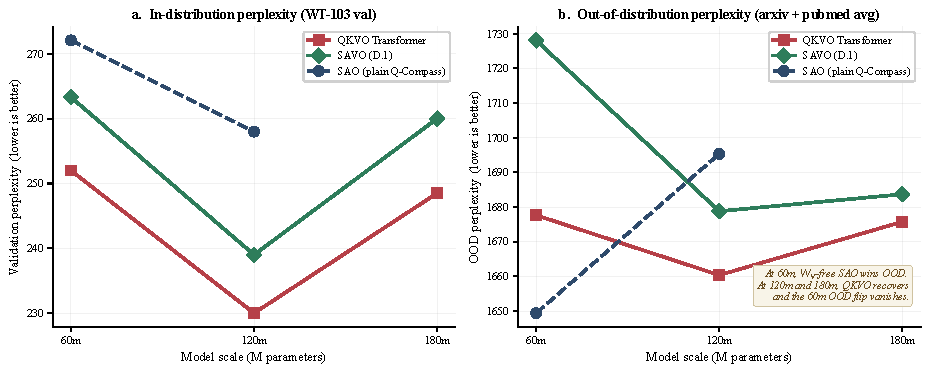
\includegraphics[width=.989\linewidth]{figs/fig08.pdf}
\caption{\textbf{In-distribution vs out-of-distribution perplexity by scale.} Panel (a): WT-103 validation perplexity; the
rank-matched transformer is best at every scale. Panel (b): average OOD perplexity on arxiv + pubmed. The 60m
$W_V$-free SAO is best; at 120m and 180m, QKVO has the lowest OOD average; SAVO and QKVO sit within $\sim$5--20
ppl on the average and within 3--5 ppl on arxiv (noise floor).}
\label{fig:8}
\end{figure}

\subsection{Cross-modal non-interference: multimodal training does not degrade text}\label{sec:5.5}

Jointly training on multiple modalities typically degrades per-token unimodal performance: in standard
multimodal stacks, the text loss at matched \emph{text}-token budget is measurably higher under the joint
schedule than under text-only training. At 60m we observe no measurable gap.

At matched \emph{optimizer} compute (10,000 steps), the multimodal model sees $\sim$ 229M text tokens (35\%
of 655M total) while the text-only model sees the full $\sim$ 655M. Interpolating the text-only training loss
curve, the text-only model reaches loss $\approx 6.31$ at step 3,500 --- the point at which it has consumed
the same $\sim$ 229M text tokens as the multimodal model at step 10,000 (text CE $= 6.328$). \textbf{At matched
text-compute, the two trajectories are indistinguishable at the per-architecture seed std measured
separately ($\boldsymbol{\sim}$0.7 ppl on val, Table~\ref{tab:5}).} Adding vision, audio, and world objectives to the shared
\QC{} stack does not measurably change the per-text-token learning rate. \emph{Caveat:} this is a single-curve,
single-observation comparison (one multimodal training run vs.\ one text-only training run, at the
matched-text-compute interpolation point). A multi-seed analogue --- multi-seed multimodal vs.\ multi-seed
text-only at matched text compute --- is deferred to future work; the SAVO multi-seed checkpoints
exist but the multimodal seeds do not.

The 120m SAVO multimodal text loss tracks the text-only trajectory at matched text-compute, and
the 180m multimodal text loss regresses in lock-step with the text-only 180m regression (Table~\ref{tab:3} vs.\
Table~\ref{tab:7}). The joint training mix is not the source of the 180m text regression --- the 10,000-step training
budget is. The non-interference observation generalises through the full 60m/120m/180m sweep.

\subsection{Scaling at text-only: 60m, 120m, 180m}\label{sec:5.6}

Table~\ref{tab:7} reports the full text-only scaling for the rank-matched transformer baseline and for SAVO. The
$h$=6 multi-head variants are reported where dimensional divisibility allows: 60m ($r$=48, $H$=384) and
180m ($r$=96, $H$=768) are clean; 120m ($r$=80, $H$=640) is not.

\begin{table}[H]
\centering
\small
\renewcommand{\arraystretch}{1.2}
\begin{tabular}{lrrrrrr}
\toprule
 & \multicolumn{2}{c}{60m} & \multicolumn{2}{c}{120m} & \multicolumn{2}{c}{180m} \\
\cmidrule(lr){2-3}\cmidrule(lr){4-5}\cmidrule(lr){6-7}
Variant & val & test & val & test & val & test \\
\midrule
Transformer QKVO, $h$=1 & \textbf{252} & 251 & \textbf{230} & --- & \textbf{248.5} & 246 \\
Transformer QKVO, $h$=6 & --- & --- & --- & --- & 258 & 255 \\
\midrule
\QC{} plain (SAO, $h$=1) & 272 & 271 & 258 & --- & --- & --- \\
MH-\QC{} (SAO, $h$=6) & 275 & 274 & --- & --- & --- & --- \\
\textbf{SAVO} ($h$=1) & \textbf{263} & 262 & \textbf{239} & 236 & \textbf{260} & 257 \\
SAVO+MH ($h$=6) & 266 & --- & --- & --- & 265 & 260 \\
\midrule
SAVO $-$ QKVO gap & +11 & +11 & +9 & +6 & +11.5 & +11 \\
\bottomrule
\end{tabular}
\caption{\textbf{Scaling across 60m / 120m / 180m (WikiText-103 perplexity; lower is better).} All models trained
10,000 steps with identical hyperparameters; single seed per cell except the 60m row, where the multi-seed paired
difference $+12.33\pm0.87$ ppl from Table~\ref{tab:5} replaces the single-seed entry. Both architectures regress 120m $\rightarrow$ 180m
at the 10,000-step budget --- a compute-budget effect, not architecture-specific. The SAVO--QKVO gap is $\sim$11--12
ppl at every scale, consistent with the 60m multi-seed mean. Multi-head adds nothing for either architecture.}
\label{tab:7}
\end{table}

\begin{figure}[H]
\centering
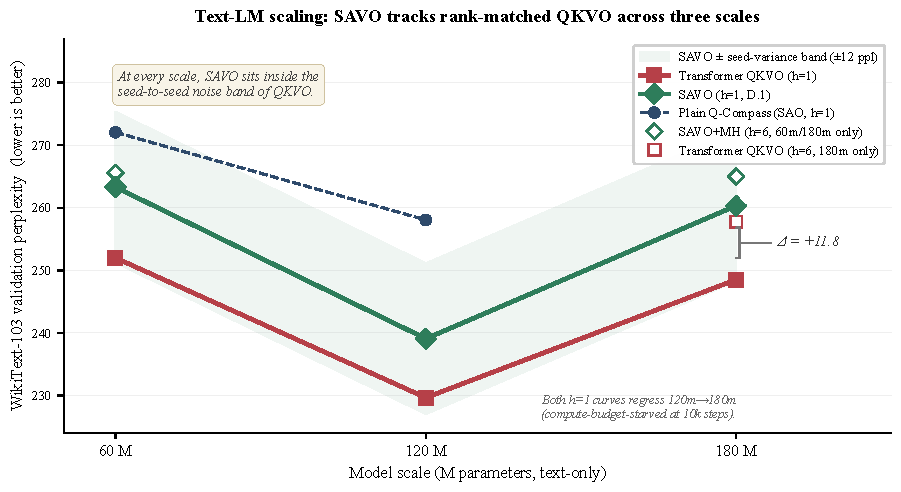
\includegraphics[width=.959\linewidth]{figs/fig09.pdf}
\caption{\textbf{SAVO tracks QKVO across 60m / 120m / 180m.} Held-out WikiText-103 val perplexity. SAVO (green
diamonds) sits $\sim$11--12 ppl above the rank-matched MHA (red squares) at every scale; the 60m gap is the multi-seed
paired difference $+12.33 \pm 0.87$ ppl ($p < 10^{-3}$, Table~\ref{tab:5}), and the 120m / 180m points are single-seed at the same
magnitude. Multi-head variants do not open a gap for either architecture at 180m. Both architectures regress
$120m \rightarrow 180m$ at a 10,000-step training budget --- a compute-budget effect, not architecture-specific.}
\label{fig:9}
\end{figure}

\subsection{60m text-LM exploratory ablation}\label{sec:5.7}

Given the 60m text-LM gap of 0.077 nats between single-head \QC{} and the rank-matched
transformer, we ran an ablation at 60m to isolate whether the gap is due to the single-head architecture,
the content-gather choice, or both. Three additional 60m runs at 33M parameters and identical training
budget: MH-QC ($h$=6, no content projection), SAVO ($h$=1, $Q$-value content), and MH-QVC ($h$=6 with
$Q$-value content).

\begin{table}[H]
\centering
\small
\renewcommand{\arraystretch}{1.2}
\begin{tabular}{lrcrr}
\toprule
Variant & Heads & $W_c$ & WT-103 val ppl & WT-103 test ppl \\
\midrule
Transformer rank-matched (QKVO) & 1 & --- & \textbf{252} & \textbf{251} \\
\midrule
\QC{} single-head (SAO) & 1 & --- & 272 & 271 \\
MH-\QC{} (SAO) & 6 & --- & 275 & 274 \\
\textbf{SAVO} (single-head) & 1 & \checkmark & \textbf{263} & \textbf{262} \\
MH-QVC & 6 & \checkmark & 266 & --- \\
\bottomrule
\end{tabular}
\caption{\textbf{60m text-LM exploratory ablation (WikiText-103).} $W_c$ closes most of the SAO$\rightarrow$QKVO gap (20
ppl $\rightarrow$ 11). Multi-head contributes nothing at 60m: per-head rank $r/h = 8$ is too small for heads to specialize.
The 180m data (Table~\ref{tab:7}) confirms multi-head remains a nothing-knob at $r/h = 16$. The structural ingredient that
matters is the $Q$-value content projection $W_c$, not the routing topology.}
\label{tab:8}
\end{table}

\subsection{SAVO compass-rank ablation at 60m}\label{sec:5.8}

We sweep the compass rank $r$ at 60m, holding all other hyperparameters fixed. The base scale config
sets $r = H/8 = 48$; we additionally train $r = H/16 = 24$ and $r = H/4 = 96$, single seed each, 10,000
optimizer steps.

\begin{table}[H]
\centering
\small
\renewcommand{\arraystretch}{1.2}
\begin{tabular}{lrrrr}
\toprule
SAVO at 60m & $r$ & $r/H$ & WT-103 val ppl & WT-103 test ppl \\
\midrule
$r = H/16$ & 24 & 0.0625 & 264.89 & 263.54 \\
$r = H/8$ & 48 & 0.125 & \textbf{263.31} & \textbf{262.46} \\
$r = H/4$ & 96 & 0.25 & 261.95 & 260.66 \\
\bottomrule
\end{tabular}
\caption{\textbf{SAVO rank ablation (60m, single seed each, 10,000 steps).} Halving the compass rank from $r$=48 to
$r$=24 raises val perplexity by 1.6; doubling to $r$=96 lowers it by 1.4. The total range across 4$\times$ rank variation
is $\sim$3 ppl. For comparison, the multi-seed per-architecture std measured at $r$=48 is 0.68 ppl (SAVO) and 0.40
ppl (rank-matched MHA, Table~\ref{tab:5}); the rank-induced differences here ($\leq$ 1.6 ppl per step) are larger than that
single-architecture std but smaller than the architectural difference ($\sim$12 ppl). SAVO appears robust to compass
rank at this scale and budget; multi-seed replication of the rank ablation is deferred to future work. Bold = the
$r = H/8$ default used everywhere else in this paper.}
\label{tab:9}
\end{table}

\subsection{Throughput, FLOPs, and memory}\label{sec:5.9}

We measure forward + backward wall-clock, peak GPU memory, and analytical attention-block FLOPs
for four attention variants at the 60m configuration ($H = 384$, $L = 1024$, batch $B = 4$), 100 timed
iterations after 5 warmup passes, on the same RTX 4050 laptop GPU used for all training in this paper.

\begin{table}[H]
\centering
\small
\resizebox{\linewidth}{!}{%
\begin{tabular}{lrrrrr}
\toprule
Attention variant & Block params & Forward (ms) & Backward (ms) & Peak GPU mem & Analytical FLOPs \\
\midrule
\QC{} (SAO, $h$=1) & 184,704 & 1.52 $\pm$ 0.04 & 2.53 $\pm$ 0.10 & 0.10 GB & 5.16 G \\
\textbf{SAVO} ($h$=1, $W_c$) & 203,136 & 1.51 $\pm$ 0.01 & 2.98 $\pm$ 0.01 & 0.11 GB & 5.31 G \\
Rank-matched MHA ($qk_r$=48, $h$=1) & 74,112 & 1.12 $\pm$ 0.01 & 2.00 $\pm$ 0.02 & 0.11 GB & 1.43 G \\
Full-rank standard MHA ($qk_r$=$H$, $h$=8) & 590,208 & 10.91 $\pm$ 0.02 & 16.28 $\pm$ 0.03 & 0.57 GB & 11.44 G \\
\bottomrule
\end{tabular}}
\caption{\textbf{Per-attention-block throughput at 60m config (RTX 4050, $\boldsymbol{L}$=1024, $\boldsymbol{B}$=4).} Mean $\pm$ std over 100
timed iterations after 5 warmup passes. \emph{Attention-block forward+backward only}: this measures the routing +
content-gather kernels in isolation; full-model wall-clock is dominated by FFN, embedding, and other components
and is not measured here. SAVO has $\sim$2.9$\times$ the parameter count of the rank-matched controlled ablation but $\sim$2.9$\times$
\emph{fewer} parameters than full-rank standard 8-head MHA, and runs $\sim$6$\times$ faster than full-rank MHA on the attention
block alone (4.5 ms vs 27.2 ms total) at $\sim$5$\times$ less peak GPU memory. Analytical FLOPs follow the same ordering.
The full-rank MHA's quadratic-in-$H$ projection cost dominates the attention-block gap; SAVO's rank-$r$ routing
avoids that cost while still using the $Q$-value content projection $W_c$ to recover most of the SAO$\rightarrow$QKVO perplexity
gap.}
\label{tab:10}
\end{table}

\subsection{Autoregressive cache footprint: SAVO is structurally rank-\texorpdfstring{$r$}{r}}\label{sec:5.10}

Standard multi-head attention requires per-token caching of $K_j = x_j W_K \in \mathbb{R}^H$ and $V_j = x_j W_V \in \mathbb{R}^H$ for
incremental decode, totalling $2H$ floats per token per layer. SAVO admits a structurally smaller cache
because both its routing key and its content are rank-$r$ quantities by construction.

\paragraph{Derivation.} Reading the SAVO forward pass (\S\ref{sec:3.1}, code at \texttt{quatrix/model.py:111\textendash118}), the only
quantities required for incremental decode at a future token $t$ are:
\begin{enumerate}
\item \textbf{Routing.} The query computes $\mathrm{softmax}(\mathrm{state}_t \cdot \mathrm{action}_j^\top/\sqrt{r})$ over cached past positions $j \leq t$. This
requires only $\mathrm{action}_j \in \mathbb{R}^r$.
\item \textbf{Content gather.} The output is $\sum_j \mathrm{weights}_{t,j} \cdot \mathrm{content}_j$ where $\mathrm{content}_j = (\mathrm{state}_j \odot \mathrm{action}_j) W_c$.
The dim-$H$ content is the projection of a dim-$r$ quantity, the elementwise product $\mathrm{qval}_j = \mathrm{state}_j \odot
\mathrm{action}_j \in \mathbb{R}^r$. Caching $\mathrm{qval}_j$ (or equivalently $\mathrm{state}_j$ and $\mathrm{action}_j$) is sufficient; the dim-$H$ content
can be reconstructed at decode time as $\mathrm{qval}_j W_c$ via a single $[L, r] \cdot [r, H]$ matmul, an $O(LrH)$ cost
that is dominated by the routing-softmax $O(L^2 r)$ cost at any $L$ for which long-context inference is
interesting.
\end{enumerate}

The total per-token per-layer cache is therefore $2r$ (state plus action, or equivalently qval plus action)
rather than $2H$. SAO does not have this property: its content is the raw $x_j \in \mathbb{R}^H$, which has rank $H$
and cannot be losslessly compressed. The structural compressibility is a property of SAVO's $Q$-value
content projection.

\begin{table}[H]
\centering
\small
\renewcommand{\arraystretch}{1.2}
\begin{tabular*}{\linewidth}{@{\extracolsep{\fill}}lrrrr@{}}
\toprule
Method & Per-token cache & At $H$=384 & 1M-context, 32-layer, fp16 & vs MHA \\
\midrule
Standard MHA ($h$=8) & $2H$ & 768 & 49\,GB & 1$\times$ \\
GQA-4 ($g$=4, $h$=8) & $2gH/h$ & 384 & 25\,GB & 0.50$\times$ \\
MQA ($h$=8) & $2H/h$ & 96 & 6.1\,GB & 0.125$\times$ \\
DeepSeek-V2 MLA \cite{ref23} & $\sim r_{\mathrm{latent}}$ & (config-dep.) & comparable regime & comparable \\
DeepSeek-V4 CSA + HCA \cite{ref18} & $\sim r_{\mathrm{latent}}$ + sparse-$k$ & (config-dep.) & 10\% of V3.2 at 1M & $\sim$0.1$\times$ \\
SAO (raw-$x$ content), $r$=$H/8$ & $H + r$ & 432 & 28\,GB & 0.56$\times$ \\
\textbf{SAVO at} $r$=$H/8$ & $2r$ & \textbf{96} & \textbf{6.1\,GB} & \textbf{0.125}$\boldsymbol{\times}$ \\
\textbf{SAVO at} $r$=$H/16$ & $2r$ & \textbf{48} & \textbf{3.1\,GB} & \textbf{0.0625}$\boldsymbol{\times}$ \\
\bottomrule
\end{tabular*}
\caption{\textbf{Autoregressive cache footprint per token per layer.} GB figures assume fp16 storage; bf16 / fp8 /
int8 inference quantisation would scale accordingly (this paper does not measure quantised inference). SAVO's
cache depends only on the compass rank $r$, not on the hidden size $H$; SAO and standard MHA scale with $H$. At
$r$=$H/8$ SAVO matches MQA's cache footprint while preserving full-rank routing across $h$ heads. At $r$=$H/16$ (val
ppl 264.89, comparable to the $r$=$H/8$ baseline per Table~\ref{tab:9}), SAVO halves MQA's footprint --- a 16$\times$ reduction
relative to standard MHA. The structural compressibility comes from SAVO's content path being a projection of a
rank-$r$ quantity (state $\odot$ action), not from any approximation or sparsification.}
\label{tab:11}
\end{table}

\paragraph{The trade-off.} SAVO at $r$=$H/8$ trades the SAVO$\rightarrow$rank-matched perplexity gap (\S\ref{sec:5.2}: $+12.33 \pm 0.87$
ppl on WikiText-103, 4-seed paired difference, $p < 10^{-3}$, Table~\ref{tab:5}) for an 8$\times$ KV-cache reduction. At
$r$=$H/16$ the cache is 16$\times$ smaller and the val-ppl penalty is at most 1.6 ppl above $r$=$H/8$ (Table~\ref{tab:9}). The
per-decode-step compute overhead of reconstructing dim-$H$ content from cached dim-$r$ qval is a single
$[L, r] \cdot [r, H]$ matmul, dominated at every interesting $L$ by the routing softmax cost. The cache reduction
is structural --- it is a consequence of SAVO's content path being intrinsically rank-$r$, not a quantization,
sparsification, or sliding-window approximation.

\paragraph{Position relative to existing work.} Multi-Query Attention \cite{ref24} reduces cache by sharing $K$ and $V$ across
all heads of standard attention; the KV cache becomes $2H/h$ at the cost of head-diversity. Grouped-Query
Attention \cite{ref9} interpolates between MHA and MQA via $g$ groups. DeepSeek-V2's Multi-head
Latent Attention \cite{ref23} compresses $K$ and $V$ into a single low-rank latent before caching; this gives a
cache footprint comparable to MQA on their configuration while preserving multi-head expressivity in
the routing. DeepSeek-V4's hybrid Compressed Sparse Attention + Heavily Compressed Attention \cite{ref18}
achieves comparable or stronger cache reduction at trillion-parameter scale through a separately introduced
compression layer plus top-$k$ sparse selection. SAVO is in the same low-rank-cache regime as
MLA and V4 but achieves it through a smaller mechanism: the routing itself operates in a rank-$r$ subspace
($Q(s, a)$ over state and action projections at rank $r$), so the cache is rank-$r$ by construction rather than by
a separately introduced compression layer or top-$k$ selector. The detailed structural relationship to V4
(developed concurrently and independently) is discussed in \S\ref{sec:6.1}.

A further consequence: SAVO's cache footprint depends only on $r$, not on $H$. Halving $r$ halves
the cache regardless of model width. Standard attention's cache scales with $H$ and so cannot reduce as
the model widens unless the head count $h$ is also raised in proportion (MQA / GQA). For long-context
applications where cache footprint per token is the dominant constraint, SAVO offers a configuration
knob ($r$) decoupled from model width and head count.
